% -*- root: main.tex -*-

%-------------------------------------------------------------------------------
\chapterimage{chapter_head_5.pdf} 

%-------------------------------------------------------------------------------
\chapter{ROS 명령어}

%-------------------------------------------------------------------------------
\section{ROS 명령어 정리}\index{ROS 명령어 정리}
\label{sec:RosCommand}

ROS는 쉘(shell)환경에서 명령어로 파일 시스템 이용, 소스코드 편집, 빌드, 디버깅, 패키지 관리 등을 처리할 수 있다. ROS를 제대로 사용하기 위해서는 기본적인 리눅스 명령어 이외에도 ROS만의 고유한 명령어\footnote{ROS, CommandLineTools, http://wiki.ros.org/ROS/CommandLineTools}들을 익힐 필요가 있다. ROS 명령어로는 다음과 같이 다양하게 존재한다. 

처음부터 모든 명령어를 숙련하게 사용할 수 없겠지만, 다음의 내용을 보고 필요할 때마다 이용하면 되겠다. 처음에는 익숙하지 않아서 불편하게 느껴질 수 있겠지만, 사용하면 사용할 수록 매우 빠르고 편하게 각종 기능을 명령어로 처리하는 자신의 모습을 보게 될 것이다.

ROS의 다양한 명령어를 숙달하기 위하여 본 강좌에서는 우선 각 명령어의 기능을 간단히 설명하고, 하나 하나 예제를 들어가며 소개하도록 하겠다. 그리고 각 명령어의 사용 빈도 및 중요도를 고려하여 필자가 별표로 점수를 매겨두었다. 별표가 많은 명령어의 경우, 사용 빈도수가 높고 중요한 명령어이니 꼭 익혀두기로 하자.

\vspace{\baselineskip}
\noindent
\textbf{[ROS 쉘 명령어]}
\begin{description}
\item[roscd] (★★★) ros+cd(changes directory) : ROS 패키지 또는 스택의 디렉토리 변경 명령어
\item[rospd] (☆☆☆) ros+pushd : ROS 디렉토리 인덱스에 디렉토리 추가
\item[rosd] (☆☆☆) ros+directory : ROS 디렉토리 인덱스 확인 명령어
\item[rosls] (★☆☆) ros+ls(lists files) : ROS 패키지의 파일 리스트를 확인하는 명령어
\item[rosed] (★☆☆) ros+ed(editor) : ROS 패키지의 파일을 편집하는 명령어
\item[roscp] (☆☆☆) ros+cp(copies files) : ROS 패키지의 파일 복사하는 명령어
\end{description}

\vspace{\baselineskip}
\noindent
\textbf{[ROS 실행 명령어]}
\begin{description}
\item[roscore] (★★★) ros+core : master (ROS 네임 서비스) + rosout (stdout/stderr) + parameter server (매개변수관리)
\item[rosrun] (★★★) ros+run : 패키지의 노드를 실행하는 명령어
\item[roslaunch] (★★★) ros+launch : 패키지의 노드를 복수개 실행하는 명령어
\item[rosclean] (★☆☆) ros+clean : ros 로그 파일을 체크하거나 삭제하는 명령어
\end{description}

\vspace{\baselineskip}
\noindent
\textbf{[ROS 정보 명령어]}
\begin{description}
\item[rostopic] (★★★) ros+topic : ROS 토픽 정보를 확인하는 명령어
\item[rosservice] (★★★) ros+service : ROS 서비스 정보를 확인하는 명령어
\item[rosnode] (★★★) ros+node : ROS의 노드 정보를 얻는 명령어
\item[rosparam] (★★★) ros+param(parameter) : ROS 파라미터 정보를 확인, 수정 가능한 명령어
\item[rosmsg] (★★☆) ros+msg : ROS 메세지 선언 정보를 확인하는 명령어
\item[rossrv] (★★☆) ros+srv : ROS 서비스 선언 정보를 확인하는 명령어
\item[roswtf] (☆☆☆) ros+wtf : ROS 시스템을 검사하는 명령어
\item[rosversion] (★☆☆) ros+version : ros 패키및 배포 릴리즈 버전의 정보를 확인하는 명령어
\item[rosbag] (★★★) ros+bag : ROS 메세지를 기록, 재생하는 명령어
\end{description}

\vspace{\baselineskip}
\noindent
\textbf{[ROS 캐킨 명령어]}
\begin{description}
\item[catkin\_create\_pkg] (★★★) 캐킨 빌드 시스템에 의한 패키지 자동 생성
\item[catkin\_eclipse] (★★☆) 캐킨 빌드 시스템에 의해 생성된 패키지를 이클립스에서 사용할 수 있도록 변경하는 명령어
\item[catkin\_find] (☆☆☆) 캐킨 검색
\item[catkin\_generate\_changelog] (☆☆☆) 캐킨 변경로그 생성
\item[catkin\_init\_workspace] (★☆☆) 캐킨 빌드 시스템의 작업폴더 초기화
\item[catkin\_make] (★★★) 캐킨 빌드 시스템을 기반으로한 빌드 명령어
\end{description}

\vspace{\baselineskip}
\noindent
\textbf{[ROS 패키지 명령어]}
\begin{description}
\item[rosmake] (☆☆☆) ros+make : ROS package 를 빌드한다. (구 ROS 빌드 시스템에서 사용됨)
\item[rosinstall] (★☆☆) ros+install : ROS 추가 패키지 설치 명령어
\item[roslocate] (☆☆☆) ros+locate : ROS 패키지 정보 관련 명령어 
\item[roscreate-pkg] (☆☆☆) ros+create-pkg : ROS 패키지를 자동 생성하는 명령어 (구 ROS 빌드 시스템에서 사용됨)
\item[rosdep] (★☆☆) ros+dep(endencies) : 해당 패키지의 의존성 파일들을 설치하는 명령어
\item[rospack] (★★☆) ros+pack(age) : ROS 패키지와 관련된 정보를 알아보는 명령어
\end{description}

%-------------------------------------------------------------------------------
\section{ROS 쉘 명령어}\index{ROS 쉘 명령어}

ROS 쉘 명령어는 일명 rosbash\footnote{ROS, rosbash, http://wiki.ros.org/rosbash}라고 부른다. 이는 리눅스에서 일반적으로 사용하는 bash 쉘 명령어를 ROS에서 사용하는 방법이다. 주로 ros 라는 접두사에 cd, pd, d, ls, ed, cp, run 등의 접미사를 붙여서 사용하게 된다. 이와 관련된 명령어들을 아래에 소개한다.  

\vspace{\baselineskip}
\noindent
\begin{description}
\item[roscd] (★★★) ros + cd (changes directory) 
\item[rospd] (☆☆☆) ros + pushd 
\item[rosd] (☆☆☆) ros + directory
\item[rosls] (★☆☆) ros + ls (lists files)
\item[rosed] (★☆☆) ros + ed (editor)
\item[roscp] (☆☆☆) ros+cp (copies files)
\item[rosrun] (★★★) ros+run 
\end{description}

\vspace{\baselineskip}
\noindent
이 중, 비교적 자주 사용되는 roscd, rosls, rosed 명령어에 대해서 자세히 알아보자.

\noindent
※ rosrun 은 rosbash 에 포함되나 의미상 ROS 실행 명령어이기 때문에 ROS 실행 명령어에서 다루도록 한다.

%-------------------------------------------------------------------------------
\subsection{roscd : ROS 디렉토리 이동}\index{roscd : ROS 디렉토리 이동}

\setcounter{num}{0}

\stepcounter{num}\circled{\thenum} 사용법
\begin{lstlisting}[language=bash]
roscd [%*패키지이름*)]
\end{lstlisting}

\noindent
\stepcounter{num}\circled{\thenum} 사용예
\begin{lstlisting}[language=bash]
$ roscd turtlesim
\end{lstlisting}

\noindent
\stepcounter{num}\circled{\thenum} 결과값
\begin{lstlisting}[language=bash]
/opt/ros/indigo/share/turtlesim$
\end{lstlisting}

\vspace{\baselineskip}
\noindent
사용예에서 처럼, turtlesim 이라는 패키지 이름을 매개변수로 넣어주고 실행하게 되면 지정된 패키지가 저장된 폴더로 이동하게 된다. 현재 결과에서는 turtlesim 이라는 패키지가 ROS가 설치되어 있는 폴더에 있으므로 위와 같이 나왔으나, 자신이 작성한 패키지의 이름을 매개변수로 넣어주면 자신이 설정한 패키지의 디렉토리로 이동할 수도 있다. 명령어 기반의 ROS를 사용하는데 있어서 매우 사용빈도가 높은 명령어이다.

\vspace{\baselineskip}
\noindent
※ 위와 같은 실행 및 결과를 위해서는 관련 패키지인 ros-indigo-turtlesim 패키지가 설치되어 있어야 한다. 만약 설치되어 있지 않은 경우 설치하도록 하자. 설치 명령어는 sudo apt-get install ros-indigo-turtlesim  이다.

%-------------------------------------------------------------------------------
\subsection{rosls : ROS 리스트 파일}\index{rosls : ROS 리스트 파일}

\setcounter{num}{0}

\stepcounter{num}\circled{\thenum} 사용법
\begin{lstlisting}[language=bash]
rosls [%*패키지이름*)]
\end{lstlisting}

\noindent
\stepcounter{num}\circled{\thenum} 사용예
\begin{lstlisting}[language=bash]
$ rosls turtlesim
\end{lstlisting}

\noindent
\stepcounter{num}\circled{\thenum} 결과값
\begin{lstlisting}[language=bash]
$ rosls turtlesim/
cmake  images  msg  package.xml  srv
\end{lstlisting}

\vspace{\baselineskip}
\noindent
지정한 ROS 패키지의 파일 리스트를 확인하는 명령어이다. roscd 명령어를 이용하여 해당 패키지로 이동후에 일반 ls 명령어로 같은 기능을 수행할 수도 있지만, 간혹 바로 확인할 필요가 있을경우에 사용된다. 사용 빈도수는 매우 떨어진다.

%-------------------------------------------------------------------------------
\subsection{rosed : ROS 편집 명령어}\index{rosed : ROS 편집 명령어}

\setcounter{num}{0}

\stepcounter{num}\circled{\thenum} 사용법
\begin{lstlisting}[language=bash]
rosed [%*패키지이름*)] [%*파일이름*)]
\end{lstlisting}

\noindent
\stepcounter{num}\circled{\thenum} 사용예
\begin{lstlisting}[language=bash]
$ rosed turtlesim package.xml 
\end{lstlisting}

\vspace{\baselineskip}
\noindent
turtlesim 패키지의 package.xml 를 편집하고자 할때 사용하는 명령어이다. 이를 실행하면 사용자가 설정한 에디터로 해당 파일을 열게된다. 급하게 간단히 파일을 수정하고자 할때 사용된다. 사용되는 에디터는 "~/.bashrc" 파일에 export EDITOR='emacs -nw' 와 같이 지정하여 사용가능하다. 필자는 비교적 단순한 편집일 경우 이를 사용한다. 프로그램 작성과 같은 작업 rosed 이외에 자신만의 개발환경을 사용하기를 추천한다.

\vspace{\baselineskip}
\noindent
\stepcounter{num}\circled{\thenum} 결과값
\begin{lstlisting}[language=bash]
%*사용자가 지정해둔 에디터를 이용하여 해당 파일을 열게된다.*)
\end{lstlisting}

\vspace{\baselineskip}
\noindent
바로 명령어창에서 수정이 필요한 단순한 작업에서 많이 사용되지만, 그 이외의 프로그램 작업등에는 비추천이다. 전체적인 사용 빈도수는 매우 떨어진다.

%-------------------------------------------------------------------------------
\section{ROS 실행 명령어}\index{ROS 실행 명령어}

ROS 실행 명령어\footnote{http://wiki.ros.org/rosbash}는 ROS 노드의 실행을 주관한다. 무엇보다 필수는 roscore로 노드간의 네임 서버로 사용된다. 그리고 실행명령어로는 rosrun 및 roslaunch가 있다. rosrun 는 하나의 노드를 실행하게 되며, roslaunch 는 하나이상의 노드를 실행할때 사용된다. 그리고 rosclean 는 노드 실행시 기록되는 로그의 삭제에 사용되는 명령어이다.

\vspace{\baselineskip}
\noindent
\begin{description}
\item[roscore] (★★★) ros+core : master (ROS 네임 서비스) + rosout (stdout/stderr) + parameter server (매개변수관리)
\item[rosrun] (★★★) ros+run : 패키지의 노드를 실행하는 명령어
\item[roslaunch] (★★★) ros+launch : 패키지의 노드를 복수개 실행하는 명령어
\item[rosclean] (★☆☆) ros+clean : ros 로그 파일을 체크하거나 삭제하는 명령어
\end{description}

%-------------------------------------------------------------------------------
\subsection{roscore : ROS 코어 실행}\index{roscore : ROS 코어 실행}
\label{subsec:Roscore}

ROS코어\footnote{http://wiki.ros.org/roscore}는 노드들간의 메시지 통신에서 연결 정보를 관리하는 마스터로서, ROS를 사용하기 위해서 제일 먼저 구동해야하는 필수 요소이다. 다음과 같이 "roscore"라는 실행 명령어로 ROS 마스터는 구동되며, XMLRPC으로 서버를 구동하게 된다. 마스터는 노드간의 접속을 위하여 노드들의 이름, 토픽 및 서비스의 이름, 메시지 형태, URI 주소 및 포트를  등록받고, 요청이 있을 경우 이 정보를 다른 노드에게 알려주는 역할을 한다. 

\setcounter{num}{0}

\vspace{\baselineskip}
\noindent
\stepcounter{num}\circled{\thenum} 사용법
\begin{lstlisting}[language=bash]
roscore [%*옵션*)]
\end{lstlisting}

\noindent
\stepcounter{num}\circled{\thenum} 사용예
\begin{lstlisting}[language=bash]
$ roscore
\end{lstlisting}

\noindent
위의 명령어로 ROS 코어를 실행하게되면 사용자가 설정해둔 ROS\_MASTER\_URI 를 마스터 URI로 하여, 마스터를 기동하게 된다. ROS\_MASTER\_URI 은 "~/.bashrc" 에서 사용자가 설정하도록 되어있다.

\vspace{\baselineskip}
\noindent
\stepcounter{num}\circled{\thenum} 결과값
\begin{lstlisting}[language=bash]
$ roscore
... logging to /home/rts/.ros/log/a42b1130-63dc-11e4-a5a1-74d02bc77892/roslaunch-rts-3547.log
Checking log directory for disk usage. This may take awhile.
Press Ctrl-C to interrupt
Done checking log file disk usage. Usage is <1GB.
started roslaunch server http://192.168.4.1:57385/
ros_comm version 1.11.9

SUMMARY
========
PARAMETERS
 * /rosdistro: indigo
 * /rosversion: 1.11.9

NODES

auto-starting new master
process[master]: started with pid [3560]
ROS_MASTER_URI=http://192.168.4.1:11311/

setting /run_id to a42b1130-63dc-11e4-a5a1-74d02bc77892
process[rosout-1]: started with pid [3575]
started core service [/rosout]
\end{lstlisting}

\vspace{\baselineskip}
\noindent
위 결과에서 /home/rt/.ros/log/ 폴더에 로그들이 저장되고 있다는 것과 "Ctrl-C" 키로 ROS 코어를 종료할 수 있다느 것, roslaunch server, ROS\_MASTER\_URI 등의 정보, /rosdistro 및 /rosversion의 파라미터 서버, /rosout 의 서비스, /rosout 노드가 실행되었음을 알수 있다.


%-------------------------------------------------------------------------------
\subsection{rosrun : ROS 노드 실행}\index{rosrun : ROS 노드 실행}

rosrun\footnote{http://wiki.ros.org/rosbash}은 지정한 패키지의 하나의 노드를 실행하는 명령어이다.

\setcounter{num}{0}

\vspace{\baselineskip}
\noindent
\stepcounter{num}\circled{\thenum} 사용법
\begin{lstlisting}[language=bash]
rosrun [%*패키지이름*)] [%*노드이름*)]
\end{lstlisting}

\noindent
\stepcounter{num}\circled{\thenum} 사용예
\begin{lstlisting}[language=bash]
$ rosrun turtlesim turtlesim_node 
\end{lstlisting}

\noindent
turtlesim 이라는 패키지의 turtlesim\_node 이라는 노드를 실행하는 명령어이다. rosrun은 지정한 패키지의 하나의 노드를 실행시킨다. 

\vspace{\baselineskip}
\noindent
\stepcounter{num}\circled{\thenum} 결과값
\begin{lstlisting}[language=bash]
$ rosrun turtlesim turtlesim_node 
[INFO] [1383445615.677782380]: Starting turtlesim with node name /turtlesim
[INFO] [1383445615.686475328]: Spawning turtle [turtle1] at x=[5.544445], y=[5.544445], theta=[0.000000]
\end{lstlisting}

\begin{figure}[h]
\centering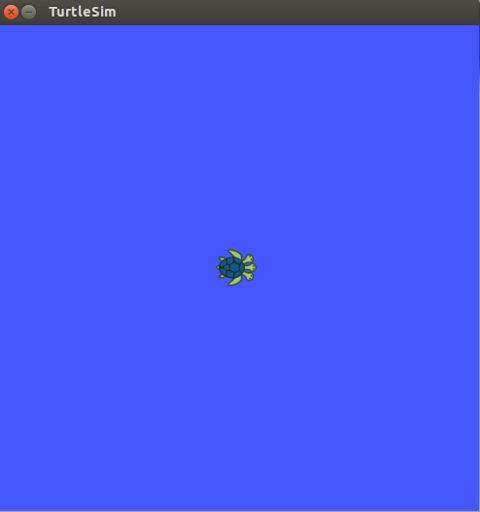
\includegraphics[width=0.6\columnwidth]{pictures/chapter5/term_rosrun.png}
\caption{turtlesim\_node 노드를 실행한 모습}
\end{figure}

%-------------------------------------------------------------------------------
\subsection{roslaunch : ROS 노드 복수 실행}\index{roslaunch : ROS 노드 복수 실행}

roslaunch\footnote{http://wiki.ros.org/roslaunch} 지정한 패키지의 하나이상의 노드를 실행하는 명령어이다. 아래와 같이 openni\_launch를 구동하는 것만으로도 camera\_nodelet\_manager, depth\_metric, depth\_metric\_rect, depth\_points 등의 20개 이상의 노드 및 10여개의 파라미터 서버가 실행된다. 이렇듯 런치파일을 이용한 실행은 하나의 패키지의 다수의 노드를 실행하는데 매우 유용하며, ROS에서는 매우 많이 사용되는 실행 방법이다. 이때 사용되는 .launch 파일 작성에 대해서는 \textbf{섹션~\ref{sec:HowToUseTheRoslaunch}~\nameref{sec:HowToUseTheRoslaunch}(pp.\pageref{sec:HowToUseTheRoslaunch})}에서 더 자세히 다루기로 하자.

\setcounter{num}{0}

\vspace{\baselineskip}
\noindent
\stepcounter{num}\circled{\thenum} 사용법
\begin{lstlisting}[language=bash]
roslaunch [%*패키지이름*)] [%*런치파일명*)]
\end{lstlisting}

\noindent
\stepcounter{num}\circled{\thenum} 사용예
\begin{lstlisting}[language=bash]
$ roslaunch openni_launch openni.launch 
\end{lstlisting}

\noindent
\stepcounter{num}\circled{\thenum} 결과값
\begin{lstlisting}[language=bash]
%*생략*)
\end{lstlisting}

※ 위와 같은 실행 및 결과를 위해서는 관련 패키지인 ros-indigo-openni-launch 패키지가 설치되어 있어야 한다. 만약 설치되어 있지 않은 경우 설치하도록 하자. 설치 명령어는 sudo apt-get install ros-indigo-openni-launch  이다.

%-------------------------------------------------------------------------------
\subsection{rosclean : ROS 로그 파일 삭제}\index{rosclean : ROS 로그 파일 삭제}

ROS 로그 파일을 체크하거나 삭제하는 명령어이다. ROS 코어(roscore)기동과 함께 모든 노드에 대한 기록은 로그파일로 기록되게 되는데 시간이 지날수록 데이타가 축척되므로 주기적으로 rosclean 명령어를 이용하여 삭제할 필요가 있다.

특히, ROS코어 실행시, "WARNING: disk usage in log directory [/xxx/.ros/log] is over 1GB." 이라는 메시지가 표시되면 로그 파일이 1기가를 초과했다는 것이므로 시스템에 무리가 예상이 된다면 rosclean 명령어를 이용하여 삭제하도록 하자.

\setcounter{num}{0}

\vspace{\baselineskip}
\noindent
\stepcounter{num}\circled{\thenum} 사용법
\begin{lstlisting}[language=bash]
rosclean [%*옵션*)]
\end{lstlisting}

\noindent
\stepcounter{num}\circled{\thenum} 사용예 (rosclean check : 로그 사용 용량 체크)
\begin{lstlisting}[language=bash]
$ roslaunch openni_launch openni.launch 
\end{lstlisting}

\noindent
\stepcounter{num}\circled{\thenum} 결과값 (rosclean check : 로그 사용 용량 체크)
\begin{lstlisting}[language=bash]
$ rosclean check
320K ROS node logs
\end{lstlisting}

\noindent
ROS 노드 로그 총 사용량이 320킬로바이트 라는 의미이다.

\vspace{\baselineskip}
\noindent
\stepcounter{num}\circled{\thenum} 사용예 (rosclean purge : 로그 삭제)
\begin{lstlisting}[language=bash]
$ rosclean purge
\end{lstlisting}

\noindent
\stepcounter{num}\circled{\thenum} 결과값 (rosclean purge : 로그 삭제)
\begin{lstlisting}[language=bash]
$ rosclean purge 
Purging ROS node logs.
PLEASE BE CAREFUL TO VERIFY THE COMMAND BELOW!
Okay to execute:
rm -rf /home/rt/.ros/log
(y/n)? y
\end{lstlisting}

\noindent
자신의 ROS 로그 저장소 (필자의 경우, /home/rt/.ros/log)의 로그를 모두 삭제할때 사용하는 명령어이다.

%-------------------------------------------------------------------------------
\section{ROS 정보 명령어}\index{ROS 정보 명령어}

ROS 정보 명령어는 토픽, 서비스, 노드, 매개변수 등의 정보를 확인하는데 사용되는 명령어로 매우 빈번히 사용되는 명령어군이다. 특히, rostopic, rosservice, rosnode, rosparam는 매우 빈번히 사용되며, rosbag 는 ROS의 큰 특징중에 하나인 데이터 기록, 재생 기능을 갖춘 명령어이므로 꼭 알아두고 활용하도록 하자.

\vspace{\baselineskip}
\noindent
\begin{description}
\item[rosnode] (★★★) ros+node : ROS 노드 관련 명령어
\item[rostopic] (★★★) ros+topic : ROS 토픽 관련 명령어
\item[rosservice] (★★★) ros+service : ROS 서비스 관련 명령어
\item[rosparam] (★★★) ros+param(parameter) : ROS 파라미터 정보를 확인, 수정 가능한 명령어
\item[rosmsg] (★★☆) ros+msg : ROS 메세지 선언 정보를 확인하는 명령어
\item[rossrv] (★★☆) ros+srv : ROS 서비스 선언 정보를 확인하는 명령어
\item[roswtf] (★☆☆) ros+wtf : ROS 시스템을 검사하는 명령어
\item[rosversion] (★☆☆) ros+version : ros 패키및 배포 릴리즈 버전의 정보를 확인하는 명령어
\item[rosbag] (★★★) ros+bag : ROS 메세지를 기록, 재생하는 명령어
\end{description}

%-------------------------------------------------------------------------------
\subsection{노드 실행}\index{노드 실행}

아래의 각 명령어를 사용하기 위해서, ROS에서 제공하는 "turtlesim" 를 이용하여 "turtlesim" 의 관련 노드, 토픽, 서비스 등을 알아 볼 것이다. ROS 정보 명령어를 이용한 테스트를 하기전에 아래처럼 "turtlesim" 관련 노드들을 미리 실행하도록 하자.

%-------------------------------------------------------------------------------
\subsubsection{roscore 실행}

원할한 따라하기식 강좌를 위해 실행 전에 기존에 실행중인 모든 터미널을 닫고 시작해 주길 바란다. 그런다음, 새로운 터미널을 열어 아래와 같은 명렁어를 실행한다. 그러면 아래와 같은 메시지를 보게 되며, 모든 노드를 관할하는 ROS코어가 실행되게 된다.

\begin{lstlisting}[language=bash]
$ roscore
\end{lstlisting}

%-------------------------------------------------------------------------------
\subsubsection{turtlesim 패키지의 turtlesim\_node 노드 실행}

좀 전과는 다른 새로운 터미널을 열어 아래와 같은 명렁어를 실행한다. 그러면 turtlesim 패키지의 turtlesim\_node를 실행하게 된다. 그러면 파란색 바탕의 화면에 거북이 한마리가 보일 것이다.

\begin{lstlisting}[language=bash]
$ rosrun turtlesim turtlesim_node 
\end{lstlisting}

%-------------------------------------------------------------------------------
\subsubsection{turtlesim 패키지의 turtle\_teleop\_key 노드 실행}

새로운 터미널을 열어 아래와 같은 명렁어를 실행한다. 그러면 turtlesim 패키지의 turtle\_teleop\_key를 실행하게 된다. 실행된 후, 이 터미널 창의 위에서 키보드의 화살표를 이용하여 거북이를 제어하게 된다. 간단하므로 직접 해보길 바란다. 제어하게 되면 화면 속의 거북이가 움직이게 되는데, 이는 간단히 시뮬레이션이지만 실제 로봇도 이와 같은 방법으로 원격조정이 가능하게 된다.

\begin{lstlisting}[language=bash]
$ rosrun turtlesim turtle_teleop_key
\end{lstlisting}

%-------------------------------------------------------------------------------
\subsection{rosnode : ROS 노드}\index{rosnode : ROS 노드}

우선, 노드(node)에 대해서 이해하고 있어야 한다. 아래 용어정리를 참고하도록 하자. 더 자세한 내용은 섹션~\nameref{sec:RosTerm}(pp.\pageref{def:RosNode})에서 설명해두었다. 참고하도록 하자.

\vspace{\baselineskip}
\noindent
\begin{description}
\item[rosnode list] : 활성화된 노드의 목록 확인
\item[rosnode ping 노드이름] : 지정된 노드와의 연결 테스트
\item[rosnode info 노드이름] : 지정된 노드의 정보 확인
\item[rosnode machine PC이름 또는 IP] : 해당 PC에서 실행되고 있는 노드 목록 확인
\item[rosnode kill 노드이름] : 지정된 노드 실행 중단
\item[rosnode cleanup] : 연결 정보가 확인 안 되는 유령 노드의 등록 정보 삭제
\end{description}

\setcounter{num}{0}

\vspace{\baselineskip}
\noindent
\stepcounter{num}\circled{\thenum} rosnode list : 활성화된 노드의 목록 확인
\begin{lstlisting}[language=ROS]
$ rosnode list
/rosout
/teleop_turtle
/turtlesim
\end{lstlisting}

\vspace{\baselineskip}
\noindent
ROS코어(roscore)에 연결된 모든 노드의 목록을 확인하는 명령어이다. 위 [사전준비] 에서 이야기한 노드만을 실행하였다면 위와 같이 roscore를 구동하면 기본적으로 시작되는 rosout 과 [사전준비]에서 실행한 /teleop\_turtle 및 /turtlesim 의 노드가 리스트에 포함되어 있음을 확인할 수 있다.

\vspace{\baselineskip}
\noindent
\stepcounter{num}\circled{\thenum} rosnode ping [노드이름] : 지정된 노드와의 연결 테스트
\begin{lstlisting}[language=ROS]
$ rosnode ping /turtlesim
rosnode: node is [/turtlesim]
pinging /turtlesim with a timeout of 3.0s
xmlrpc reply from http://192.168.4.185:45470/ time=0.854969ms
\end{lstlisting}

\vspace{\baselineskip}
\noindent
위 명령어는 /turtlesim 노드가 실제로 현재 사용중인 컴퓨터와 연결이 되어 있는지에 대한 테스트이다. 만약에 해당 노드와 연결되어 있지 않으면 "ERROR: connection refused to [http://192.168.4.185:55996/]" 와 같은 에러 메세지를 보게될 것이다.

\vspace{\baselineskip}
\noindent
\stepcounter{num}\circled{\thenum} rosnode info [노드이름] : 지정된 노드의 정보 확인
\begin{lstlisting}[language=ROS]
$ rosnode info /turtlesim 
--------------------------------------------------------------------------------
Node [/turtlesim]
Publications: 
 * /turtle1/color_sensor [turtlesim/Color]
...
\end{lstlisting}

\vspace{\baselineskip}
\noindent
rosnode info 명령어를 이용하면 지정한 노드의 정보를 확인가능하다. 기본적으로, Publications, Subscriptions, Services 등을 확인할 수 있으며, 노드 실행 URI 및 토픽 입출력에 대한 정보들도 확인 가능하다. 많은 정보 출력으로 위에서는 내용을 생략해 두었으므 꼭 실행해보길 권장한다.

\vspace{\baselineskip}
\noindent
\stepcounter{num}\circled{\thenum} rosnode machine [PC이름 또는 IP] : 해당 PC에서 실행되고 있는 노드 목록 확인
\begin{lstlisting}[language=ROS]
$ rosnode machine 192.168.4.185
/rosout
/teleop_turtle
/turtlesim
\end{lstlisting}

\vspace{\baselineskip}
\noindent
지정된 특정 머신(PC 및 단말기)에서 작동죽인 노드의 목록을 확인할 수 있다.

\vspace{\baselineskip}
\noindent
\stepcounter{num}\circled{\thenum} rosnode kill [노드이름] : 지정된 노드 실행 종료
\begin{lstlisting}[language=ROS]
$ rosnode kill /turtlesim
killing /turtlesim
killed
\end{lstlisting}

\vspace{\baselineskip}
\noindent
실행중인 노드를 종료하는 명령어이다. 노드가 실행된 터미널창에서 Ctrl + C 를 이용하여 직접 노드를 종료할 수도 있지만, 이렇게 해당 노드를 지정하여 종료할 수도 있다. 만약 이 명령어로 종료하게 되면 아래와 같이 해당 노드가 실행중인 터미널에 경고 메시지가 출력되면서 해당 노드는 종료되게 된다.

\begin{lstlisting}[language=ROS]
[ WARN] [1383455647.514022654]: Shutdown request received.
[ WARN] [1383455647.514058274]: Reason given for shutdown: [user request]
\end{lstlisting}

\vspace{\baselineskip}
\noindent
\stepcounter{num}\circled{\thenum} rosnode cleanup : 연결 정보가 확인안되는 유령 노드의 등록 정보 삭제
\begin{lstlisting}[language=ROS]
$ rosnode cleanup 
\end{lstlisting}

\vspace{\baselineskip}
\noindent
연결 정보가 확인안되는 유령 노드의 등록 정보를 삭제한다. 예기치못한 일로 노드가 비정상적으로 종료된경우, 이 명령어로 연결 정보가 끓어진 노드를 목록에서 삭제하게된다. 간혹 사용되지만 roscore 을 재실행하는 일이 없기에 매우 유용한 명령어이다.


%-------------------------------------------------------------------------------
\subsection{rostopic : ROS 토픽}\index{rostopic : ROS 토픽}

우선, 토픽(topic)에 대해서 이해하고 있어야 한다. 아래 용어정리를 참고하도록 하자. 더 자세한 내용은 섹션~\nameref{sec:RosTerm}(pp.\pageref{def:RosTopic})에서 설명해두었다. 참고하도록 하자.

\vspace{\baselineskip}
\noindent
\begin{description}
\item[rostopic list] : 활성화된 토픽의 목록을 표시한다
\item[rostopic echo 토픽이름] : 지정한 토픽의 메시지 내용을 실시간으로 표시한다
\item[rostopic find 타입이름] : 지정한 타입의 메시지를 사용하는 토픽을 표시한다
\item[rostopic type 토픽이름] : 지정한 토픽의 메시지 타입을 표시한다
\item[rostopic bw 토픽이름] : 지정한 토픽의 메시지 데이터 대역폭(bandwidth)을 표시한다
\item[rostopic hz 토픽이름] : 지정한 토픽의 메세지 데이터 발행주기를 표시한다
\item[rostopic info 토픽이름] : 지정한 토픽의 정보를 표시한다
\item[rostopic pub 토픽이름 메시지타입 매개변수] : 지정한 토픽의 이름으로 메시지를 발행한다
\end{description}

\vspace{\baselineskip}
\noindent
※ 아래의 예제를 실행하기 전에 모든 노드를 종료하도록 하자. 그리고 난후, 각각 다른 터미널창에서 아래의 명령어를 실행하여 turtlesim\_node 및 turtle\_teleop\_key를 실행해주자.

\begin{lstlisting}[language=ROS]
roscore
rosrun turtlesim turtlesim_node 
rosrun turtlesim turtle_teleop_key
\end{lstlisting}

\setcounter{num}{0}

\vspace{\baselineskip}
\noindent
\stepcounter{num}\circled{\thenum} rostopic list : 활성화된 토픽의 목록을 표시한다

\begin{lstlisting}[language=ROS]
$ rostopic list
/rosout
/rosout_agg
/turtle1/cmd_vel
/turtle1/color_sensor
/turtle1/pose
\end{lstlisting}

\noindent
rostopic list 명령어는 현재 송신 및 수신되고 있는 모든 토픽의 리스트를 확인할 수 있게 해준다.

\begin{lstlisting}[language=ROS]
$ rostopic list -v

Published topics:
 * /turtle1/color_sensor [turtlesim/Color] 1 publisher
 * /turtle1/cmd_vel [geometry_msgs/Twist] 1 publisher
 * /rosout [rosgraph_msgs/Log] 2 publishers
 * /rosout_agg [rosgraph_msgs/Log] 1 publisher
 * /turtle1/pose [turtlesim/Pose] 1 publisher

Subscribed topics:
 * /turtle1/cmd_vel [geometry_msgs/Twist] 1 subscriber
 * /rosout [rosgraph_msgs/Log] 1 subscriber
\end{lstlisting}

\noindent
rostopic list 명령어에 -v 이라는 옵션을 추가해주면, 발행되고 있는 토픽 및 수신되고 있는 토픽을 나누어 주고, 각 토픽의 메시지 타입까지 함께 표시해준다.

\vspace{\baselineskip}
\noindent
\stepcounter{num}\circled{\thenum} rostopic echo [토픽이름] : 지정한 토픽의 메시지 내용을 실시간으로 표시한다.

\begin{lstlisting}[language=ROS]
$ rostopic echo /turtle1/pose 
x: 5.35244464874
y: 5.544444561
theta: 0.0
linear_velocity: 0.0
angular_velocity: 0.0
---
...
\end{lstlisting}

\noindent
/turtle1/pose 토픽을 구성하는 x, y, theta, linear\_velocity, angular\_velocity 의 데이터를 실시간으로 확인할 수 있다.

\vspace{\baselineskip}
\noindent
\stepcounter{num}\circled{\thenum} rostopic find [타입이름] : 지정한 타입의 메시지를 사용하는 토픽을 표시한다

\begin{lstlisting}[language=ROS]
$ rostopic find turtlesim/Pose
/turtle1/pose
\end{lstlisting}

\vspace{\baselineskip}
\noindent
\stepcounter{num}\circled{\thenum} rostopic type [토픽이름] : 지정한 토픽의 메시지 타입을 표시한다

\begin{lstlisting}[language=ROS]
$ rostopic type /turtle1/pose 
turtlesim/Pose
\end{lstlisting}

\vspace{\baselineskip}
\noindent
\stepcounter{num}\circled{\thenum} rostopic bw [토픽이름] : 지정한 토픽의 메시지 데이터 대역폭(bandwidth)을 표시한다

\begin{lstlisting}[language=ROS]
$ rostopic bw /turtle1/pose 
subscribed to [/turtle1/pose]
average: 1.27KB/s
 mean: 0.02KB min: 0.02KB max: 0.02KB window: 62
...
\end{lstlisting}

\noindent
/turtle1/pose 토픽에 사용되는 데이터 대역폭은 초당 1.27KB 임을 확인할 수 있다.

\vspace{\baselineskip}
\noindent
\stepcounter{num}\circled{\thenum} rostopic hz [토픽이름] : 지정한 토픽의 메세지 데이터 발행주기를 표시한다

\begin{lstlisting}[language=ROS]
$ rostopic hz /turtle1/pose 
subscribed to [/turtle1/pose]
average rate: 62.502
 min: 0.016s max: 0.016s std dev: 0.00005s window: 62
\end{lstlisting}

\noindent
/turtle1/pose 의 데이타의 발행 주기를 확인해 볼 수 있다. 위의 결과로는 약 62.5Hz (0.016초=16msec) 주기로 메시지가 발행되고 있음을 알 수 있다.

\vspace{\baselineskip}
\noindent
\stepcounter{num}\circled{\thenum} rostopic info [토픽이름] : 지정한 토픽의 정보를 표시한다

\begin{lstlisting}[language=ROS]
$ rostopic info /turtle1/pose 
Type: turtlesim/Pose
Publishers: 
 * /turtlesim (http://192.168.4.185:42443/)
Subscribers: None
\end{lstlisting}

\noindent
/turtle1/pose 토픽은 turtlesim/Pose 메시지 타입을 사용하고 있고, /turtlesim 노드에 발행되고 있으며, 구독되고 있는 토픽은 없다는 정보를 확인할 수 있다. 

\vspace{\baselineskip}
\noindent
\stepcounter{num}\circled{\thenum} rostopic pub [토픽이름] [메시지타입] [매개변수] : 지정한 토픽의 이름으로 메시지를 발행한다

\begin{lstlisting}[language=ROS]
$ rostopic pub -1 /turtle1/cmd_vel geometry_msgs/Twist -- '[2.0, 0.0, 0.0]' '[0.0, 0.0, 1.8]'
publishing and latching message for 3.0 seconds
\end{lstlisting}

\noindent
/turtle1/pose 토픽은 turtlesim/Pose 메시지 타입을 사용하고 있고, /turtlesim 노드에 발행되고 있으며, 구독되고 있는 토픽은 없다는 정보를 확인할 수 있다. 

\vspace{\baselineskip}
\noindent
\textbf{[옵션 값 지정에 대한 설명]}
\begin{itemize}[leftmargin=*]
\item \textbf{-1} : 메시지를 1번만 발행한다. (실제로는 1번 실행이기는 하지만 위의 결과처럼 3초간 실행된다.)
\item \textbf{/turtle1/cmd\_vel} : 지정한 토픽이름
\item \textbf{geometry\_msgs/Twist} : 발행되는 메시지 타입 이름
\item \textbf{-- '[2.0, 0.0, 0.0]' '[0.0, 0.0, 1.8]'} : x축 좌표로 초당 2.0 미터(m/s)의 속도 이동, z축 좌표로 초당 1.8 라디안 (radian/s) 회전을 하라는 값이다.
\end{itemize}

\begin{figure}[h]
\centering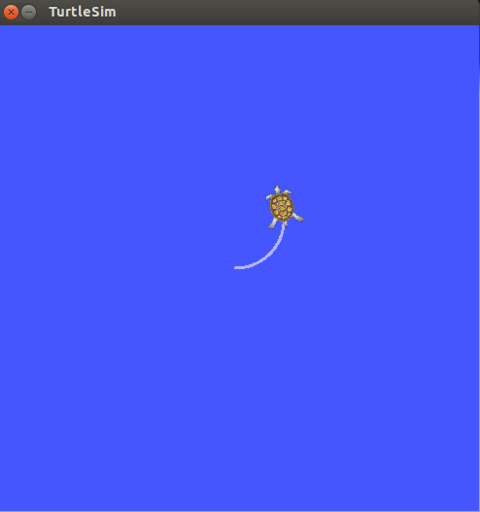
\includegraphics[width=0.7\columnwidth]{pictures/chapter5/rostopic_pub.png}
\caption{발행된 메시지가 반영된 모습}
\end{figure}


%-------------------------------------------------------------------------------
\subsection{rosservice : ROS 서비스}\index{rosservice : ROS 서비스}

우선, 서비스(service)\footnote{ROS, rosservice, http://wiki.ros.org/rosservice}에 대해서 이해하고 있어야 한다. 아래 용어정리를 참고하도록 하자. 더 자세한 내용은 섹션~\nameref{sec:RosTerm}(pp.\pageref{def:RosService})에서 설명해두었다. 참고하도록 하자.

\vspace{\baselineskip}
\noindent
\begin{description}
\item[rosservice list] : 활성화된 서비스에 대한 정보를 출력한다
\item[rosservice type 서비스이름] : 서비스 타입을 출력한다
\item[rosservice find 서비스타입] : 지정한 서비스 타입의 서비스를 검색한다
\item[rosservice uri  서비스이름] : ROSRPC uri 서비스를 출력한다
\item[rosservice args 서비스이름] : 서비스 매개변수 출력
\item[rosservice call 서비스이름 매개변수] : 입력된 매개변수로 서비스를 요청한다
\end{description}

\vspace{\baselineskip}
\noindent
※ 아래의 예제를 실행하기 전에 모든 노드를 종료하도록 하자. 그리고 난후, 각각 다른 터미널창에서 아래의 명령어를 실행하여 turtlesim\_node 및 turtle\_teleop\_key를 실행해주자.

\begin{lstlisting}[language=ROS]
roscore
rosrun turtlesim turtlesim_node 
rosrun turtlesim turtle_teleop_key
\end{lstlisting}

\setcounter{num}{0}

\vspace{\baselineskip}
\noindent
\stepcounter{num}\circled{\thenum} rosservice list : 활성화된 서비스에 대한 정보를 출력한다

\begin{lstlisting}[language=ROS]
$ rosservice list
/clear
/kill
/reset
/rosout/get_loggers
/rosout/set_logger_level
/spawn
/teleop_turtle/get_loggers
/teleop_turtle/set_logger_level
/turtle1/set_pen
/turtle1/teleport_absolute
/turtle1/teleport_relative
/turtlesim/get_loggers
/turtlesim/set_logger_level
\end{lstlisting}

\noindent
동일한 네트워크에서 사용중인 서비스가 모두 표시된다.

\vspace{\baselineskip}
\noindent
\stepcounter{num}\circled{\thenum} rosservice type [서비스이름] : 서비스 타입을 출력한다.

\begin{lstlisting}[language=ROS]
$ rosservice type /turtle1/set_pen
turtlesim/SetPen
\end{lstlisting}

\noindent
/turtle1/set\_pen 서비스는 turtlesim/SetPen 형태의 서비스 타입임을 확인할 수 있다.

\vspace{\baselineskip}
\noindent
\stepcounter{num}\circled{\thenum} rosservice find [서비스타입] : 지정한 서비스 타입의 서비스를 검색한다

\begin{lstlisting}[language=ROS]
$ rosservice find turtlesim/SetPen
/turtle1/set_pen
\end{lstlisting}

\noindent
"turtlesim/SetPen" 형태의 서비스 타입의 서비스를 검색하는 명령어이다. 결과로는 "/turtle1/set\_pen" 가 나왔음을 확인할 수 있다.

\vspace{\baselineskip}
\noindent
\stepcounter{num}\circled{\thenum} rosservice uri [서비스이름] : ROSRPC uri 서비스를 출력한다

\begin{lstlisting}[language=ROS]
$ rosservice uri /turtle1/set_pen
rosrpc://192.168.4.185:49714
\end{lstlisting}

\noindent
"/turtle1/set\_pen" 서비스의 ROSRPC uri를 확인할 수 있다.

\vspace{\baselineskip}
\noindent
\stepcounter{num}\circled{\thenum} rosservice args [서비스이름] : 서비스 매개변수 출력

\begin{lstlisting}[language=ROS]
$ rosservice args /turtle1/set_pen
r g b width off
\end{lstlisting}

\noindent
"/turtle1/set\_pen" 서비스의 각 매개변수를 확인할 수 있다. 위의 명령어에서는 r, g, b, width, off 라는 매개변수가 사용됨을 확인할 수 있었다.

\vspace{\baselineskip}
\noindent
\stepcounter{num}\circled{\thenum}  rosservice call [서비스이름] [매개변수] : 입력된 매개변수로 서비스를 요청한다

\begin{lstlisting}[language=ROS]
$ rosservice call /turtle1/set_pen 255 0 0 5 0
\end{lstlisting}

\noindent
"/turtle1/set\_pen" 서비스를 요청하는 명령어이다. 사용된 255 0 0 5 0 은 "/turtle1/set\_pen" 서비스에 사용되는 매개변수(r, g, b, width, off)에 해당되는 수치이다.  빨간색의 r의 최대치인 255으로 하고, g,b 는 모두 0 이므로 펜의 색깔을 빨간색으로 설정하라는 이야기이며, width는 5의 굵기로 설정, off는 0(false)이기에 선이 보이도록 하는것을 의미한다. 그 결과가 아래와 같다. 위 명령어로 서비스를 요청하여 TurtleSim에 사용되는 펜의 특성을 바꾸었고, turtle\_teleop\_key에서 명령을 내려 이동한 결과 아래와 같이 흰색이였던 펜 색이 빨간색으로 표시됨을 확인할 수 있다.

\begin{figure}[h]
\centering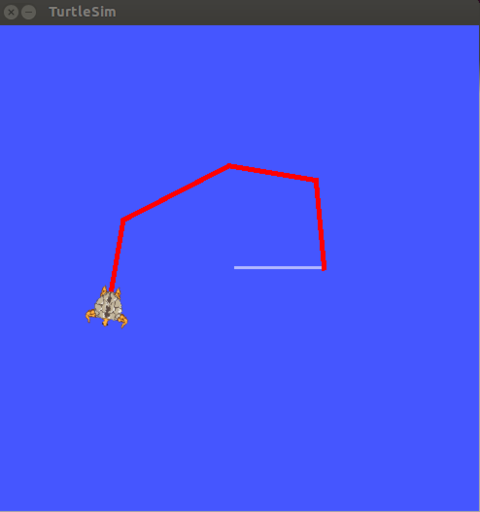
\includegraphics[width=0.5\columnwidth]{pictures/chapter5/rosservice_call.png}
\caption{rosservice call 예제}
\end{figure}

%-------------------------------------------------------------------------------
\subsection{rosparam : ROS 매개변수}\index{rosparam : ROS 매개변수}

우선, 매개변수(parameter)\footnote{ROS, rosparam, http://wiki.ros.org/rosparam}에 대해서 이해하고 있어야 한다. 자세한 내용은 섹션~\nameref{sec:RosTerm}(pp.\pageref{def:RosParameter})에서 설명해두었다. 참고하도록 하자.

\vspace{\baselineskip}
\noindent
\begin{description}
\item[rosparam list] : 매개변수 목록 보기
\item[rosparam get 매개변수이름] : 매개변수 값 불러오기
\item[rosparam set 매개변수이름] : 매개변수 값 설정 
\item[rosparam dump 파일이름] : 매개변수를 지정한 파일에 저장한다
\item[rosparam load 파일이름] : 지정한 파일에 저장된 매개변수를 불러온다
\item[rosparam delete 매개변수이름] : 매개변수를 삭제한다 
\end{description}

\vspace{\baselineskip}
\noindent
※ 아래의 예제를 실행하기 전에 모든 노드를 종료하도록 하자. 그리고 난후, 각각 다른 터미널창에서 아래의 명령어를 실행하여 turtlesim\_node 및 turtle\_teleop\_key를 실행해주자.

\begin{lstlisting}[language=ROS]
roscore
rosrun turtlesim turtlesim_node 
rosrun turtlesim turtle_teleop_key
\end{lstlisting}

\setcounter{num}{0}

\vspace{\baselineskip}
\noindent
\stepcounter{num}\circled{\thenum} rosparam list : 매개변수 목록 보기

\begin{lstlisting}[language=ROS]
$ rosparam list
/background_b
/background_g
/background_r
/rosdistro
/roslaunch/uris/host_192_168_4_185__39536
/rosversion
/run_id
\end{lstlisting}

\noindent
동일한 네트워크에서 사용중인 매개변수 목록이 표시된다.

\vspace{\baselineskip}
\noindent
\stepcounter{num}\circled{\thenum} rosparam get [매개변수이름] : 매개변수 값 불러오기

\begin{lstlisting}[language=ROS]
$ rosparam get /background_b
255
\end{lstlisting}

\noindent
특정 매개변수 값을 확인하고 싶을때는 위와 같이 "rosparam get" 명령어에 옵션으로 매개변수이름을 적어주면 된다.

\begin{lstlisting}[language=ROS]
$ rosparam get /
background_b: 255
background_g: 86
background_r: 69
rosdistro: 'hydro
  '
roslaunch:
  uris: {host_192_168_4_185__39536: 'http://192.168.4.185:39536/'}
rosversion: '1.9.50
  '
run_id: 93598b26-44f6-11e3-a077-d43d7e970cb0
\end{lstlisting}

\noindent
특정 매개변수가 아니라 모든 매개변수의 값을 확인하고 싶을 경우에는 옵션으로 "/" 를 붙여주면 위와같이 모든 매개변수의 값을 확인할 수 있다.

\vspace{\baselineskip}
\noindent
\stepcounter{num}\circled{\thenum} rosparam set [매개변수이름] : 매개변수 값 설정 

\begin{lstlisting}[language=ROS]
$ rosparam set background_b 0
$ rosservice call clear
\end{lstlisting}

\begin{figure}[h]
\centering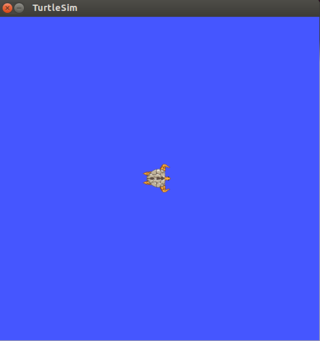
\includegraphics[width=0.4\columnwidth]{pictures/chapter5/rosparam_set1.png}
\centering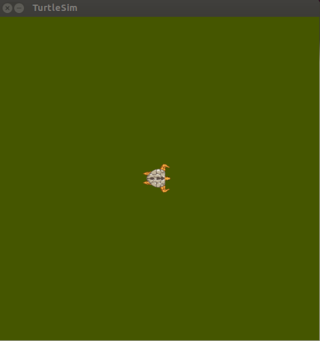
\includegraphics[width=0.4\columnwidth]{pictures/chapter5/rosparam_set2.png}
\caption{rosparam set 예제}
\end{figure}

\noindent
매개변수 값을 설정하는 명령어이다. 위 예제에서 "turtlesim" 노드의 배경색관련 매개변수인 "background\_b" 를 "0"으로 설정하였다. 그러면 rgb 는 255, 86, 69 에서 0, 86, 69 으로 변경되기에 위 오른쪽 그림처럼 짙은 녹색이 된다.

단, "turtlesim" 노드는 매개변수를 매번 읽는 것이 아니기에 "rosparam set background\_b 0" 명령어로 매개변수를 수정후에, "rosservice call clear" 명령어로 화면을 갱신해줘야한다. 이는 노드에 따라 매개변수 반영이 달라지게 된다.

\vspace{\baselineskip}
\noindent
\stepcounter{num}\circled{\thenum} rosparam dump [파일이름] : 매개변수를 지정한 파일에 저장한다

\begin{lstlisting}[language=ROS]
$ rosparam dump ~/parameters.yaml
\end{lstlisting}

\noindent
현재의 매개변수 값을 "parameters.yaml" 라는 파일에 저장하게 된다. 이는 매번 사용되는 매개변수값을 저장하여 다음 실행때에 사용할 수 있어서 매우 편리하다. (~/ 은 유저의 home 폴더를 의미한다)

\vspace{\baselineskip}
\noindent
\stepcounter{num}\circled{\thenum} rosparam delete [매개변수이름] : 매개변수를 삭제한다

\begin{lstlisting}[language=ROS]
$ rosparam delete /background_b
\end{lstlisting}

\noindent
지정한 매개변수를 삭제하는 명령어이다.

%-------------------------------------------------------------------------------
\subsection{rosmsg : ROS 메시지 정보}\index{rosmsg : ROS 메시지 정보}

우선, 메시지(message)\footnote{ROS, rosmsg, http://wiki.ros.org/rosmsg}에 대해서 이해하고 있어야 한다. 자세한 내용은 섹션~\nameref{sec:RosTerm}(pp.\pageref{def:RosMessage})에서 설명해두었다. 참고하도록 하자.

\vspace{\baselineskip}
\noindent
\begin{description}
\item[rosmsg list] : 모든 메시지를 목록으로 표시한다
\item[rosmsg show 메시지이름] : 지정한 메시지 정보를 표시한다
\item[rosmsg md5 메시지이름] : md5sum을 표시한다
\item[rosmsg package 패키지이름] : 지정한 패키지에서 사용되는 메시지의 목록을 표시한다
\item[rosmsg packages] : 메시지를 사용하는 모든 패키지의 목록을 표시한다
\end{description}

\vspace{\baselineskip}
\noindent
※ 아래의 예제를 실행하기 전에 모든 노드를 종료하도록 하자. 그리고 난후, 각각 다른 터미널창에서 아래의 명령어를 실행하여 turtlesim\_node 및 turtle\_teleop\_key를 실행해주자.

\begin{lstlisting}[language=ROS]
roscore
rosrun turtlesim turtlesim_node 
rosrun turtlesim turtle_teleop_key
\end{lstlisting}

\setcounter{num}{0}

\vspace{\baselineskip}
\noindent
\stepcounter{num}\circled{\thenum} rosmsg list : 모든 메시지를 목록으로 표시한다

\begin{lstlisting}[language=ROS]
$ rosmsg list
actionlib/TestAction
actionlib/TestActionFeedback
actionlib/TestActionGoal
actionlib/TestActionResult
actionlib/TestFeedback
actionlib/TestGoal
actionlib/TestRequestAction
actionlib/TestRequestActionFeedback
actionlib/TestRequestActionGoal
actionlib/TestRequestActionResult
...
\end{lstlisting}

\noindent
현재 ROS에 포함되어 있는 패키지에 따라 결과값이 틀려질 수 있다. 이 명령어는 현재 ROS에 설치된 패키지의 모든 메시지를 목록으로 표시하게 된다.

\vspace{\baselineskip}
\noindent
\stepcounter{num}\circled{\thenum} rosmsg show [메시지이름] : 지정한 메시지 정보를 표시한다

\begin{lstlisting}[language=ROS]
$ rosmsg show turtlesim/Pose 
float32 x
float32 y
float32 theta
float32 linear_velocity
float32 angular_velocity
\end{lstlisting}

\noindent
지정한 메시지 정보를 표시한다. 위 예제에서는 "turtlesim/Pose" 라는 이름의 메시지의 정보를 출력해보았다. float32 부동소수점형 변수로 x, y, theta, linear\_velocity, angular\_velocity 의 5개의 정보가 포함되어 있는 메시지임을 확인할 수 있다.

\vspace{\baselineskip}
\noindent
\stepcounter{num}\circled{\thenum} rosmsg md5 [메시지이름] : md5sum\footnote{섹션~\nameref{sec:RosTerm}(pp.\pageref{def:RosMD5})}을 표시한다

\begin{lstlisting}[language=ROS]
$ rosmsg md5 turtlesim/Pose 
863b248d5016ca62ea2e895ae5265cf9
\end{lstlisting}

\noindent
"turtlesim/Pose" 라는 이름의 메시지의 md5 정보를 확인한다. 간혹 메시지 통신중에 MD5 문제가 발생된다면 md5sum 을 확인할 필요가 있는데 이때에 사용되는 명령어이다. 일반적으로 많이 사용되지는 않는다.

\vspace{\baselineskip}
\noindent
\stepcounter{num}\circled{\thenum} rosmsg package [패키지이름] : 지정한 패키지에서 사용되는 메시지의 목록을 표시한다

\begin{lstlisting}[language=ROS]
$ rosmsg package turtlesim 
turtlesim/Color
turtlesim/Pose
\end{lstlisting}

\noindent
특정 패키지에서 사용되는 메시지들을 확인할 수 있다.

\vspace{\baselineskip}
\noindent
\stepcounter{num}\circled{\thenum} rosmsg packages : 메시지를 사용하는 모든 패키지의 목록을 표시한다

\begin{lstlisting}[language=ROS]
$ rosmsg packages
actionlib
actionlib_msgs
actionlib_tutorials
base_local_planner
bond
control_msgs
costmap_2d
\end{lstlisting}

%-------------------------------------------------------------------------------
\subsection{rossrv : ROS 서비스 정보}\index{rossrv : ROS 서비스 정보}

우선, 서비스(service)\footnote{ROS, rosmsg, http://wiki.ros.org/rosmsg}에 대해서 이해하고 있어야 한다. 자세한 내용은 섹션~\nameref{sec:RosTerm}(pp.\pageref{def:RosService})에서 설명해두었다. 참고하도록 하자.

\vspace{\baselineskip}
\noindent
\begin{description}
\item[rossrv list] : 모든 서비스를 목록으로 표시한다
\item[rossrv show 서비스이름] : 지정한 서비스 정보를 표시한다
\item[rossrv md5 서비스이름] : md5sum을 표시한다
\item[rossrv package 패키지이름] : 지정한 패키지에서 사용되는 서비스의 목록을 표시한다
\item[rossrv packages] : 서비스를 사용하는 모든 패키지의 목록을 표시한다
\end{description}

\vspace{\baselineskip}
\noindent
※ 아래의 예제를 실행하기 전에 모든 노드를 종료하도록 하자. 그리고 난후, 각각 다른 터미널창에서 아래의 명령어를 실행하여 turtlesim\_node 및 turtle\_teleop\_key를 실행해주자.

\begin{lstlisting}[language=ROS]
roscore
rosrun turtlesim turtlesim_node 
rosrun turtlesim turtle_teleop_key
\end{lstlisting}

\setcounter{num}{0}

\vspace{\baselineskip}
\noindent
\stepcounter{num}\circled{\thenum} rossrv list : 모든 서비스를 목록으로 표시한다

\begin{lstlisting}[language=ROS]
$ rossrv list
control_msgs/QueryCalibrationState
control_msgs/QueryTrajectoryState
diagnostic_msgs/SelfTest
dynamic_reconfigure/Reconfigure
gazebo_msgs/ApplyBodyWrench
gazebo_msgs/ApplyJointEffort
gazebo_msgs/BodyRequest
gazebo_msgs/DeleteModel
...
\end{lstlisting}

\noindent
현재 ROS에 포함되어 있는 패키지에 따라 결과값이 틀려질 수 있다. 이 명령어는 현재 ROS에 설치된 패키지의 모든 서비스를 목록으로 표시하게 된다.

\vspace{\baselineskip}
\noindent
\stepcounter{num}\circled{\thenum} rossrv show [서비스이름] : 지정한 서비스 정보를 표시한다

\begin{lstlisting}[language=ROS]
$ rossrv md5 turtlesim/SetPen 
9f452acce566bf0c0954594f69a8e41b
\end{lstlisting}

\noindent
"turtlesim/SetPen" 라는 이름의 서비스의 md5 정보를 확인한다. 간혹 서비스 요청 중에 MD5 문제가 발생된다면 md5sum 을 확인할 필요가 있는데 이때에 사용되는 명령어이다. 일반적으로 많이 사용되지는 않는다.

\vspace{\baselineskip}
\noindent
\stepcounter{num}\circled{\thenum} rossrv package [패키지이름] : 지정한 패키지에서 사용되는 서비스의 목록을 표시한다

\begin{lstlisting}[language=ROS]
$ rossrv package turtlesim 
turtlesim/Kill
turtlesim/SetPen
|turtlesim/Spawn
turtlesim/TeleportAbsolute
turtlesim/TeleportRelative
\end{lstlisting}

\noindent
특정 패키지에서 사용되는 메시지들을 확인할 수 있다.

\vspace{\baselineskip}
\noindent
\stepcounter{num}\circled{\thenum} rossrv packages : 서비스를 사용하는 모든 패키지의 목록을 표시한다

\begin{lstlisting}[language=ROS]
$ rossrv packages
control_msgs
diagnostic_msgs
dynamic_reconfigure
gazebo_msgs
laser_assembler
map_msgs
nav_msgs
navfn
nodelet
oroca_ros_tutorials
polled_camera
robot_pose_ekf
roscpp
roscpp_tutorials
rospy_tutorials
sensor_msgs
std_srvs
tf
tf2_msgs
topic_tools
turtlesim
\end{lstlisting}

%-------------------------------------------------------------------------------
\subsection{rosbag : ROS 로그 정보}\index{rosbag : ROS 로그 정보}
\label{subsub:Rosbag}

우선, 배그(bag)\footnote{ROS, rosbag, http://wiki.ros.org/rosbag}\footnote{ROS, Bags Format, http://wiki.ros.org/Bags/Format}에 대해서 이해하고 있어야 한다. 자세한 내용은 섹션~\nameref{sec:RosTerm}(pp.\pageref{def:RosBag})에서 설명해두었다. 참고하도록 하자.

\vspace{\baselineskip}
\noindent
\begin{description}
\item[rosbag record 옵션 토픽이름] : 지정한 토픽의 메시지를 기록한다
\item[rosbag info bag파일이름] : 배그파일의 정보를 확인한다
\item[rosbag play bag파일이름] : 지정한 배그파일을 재생한다

\item[rosbag compress bag파일이름] : 지정한 배그파일을 압축한다
\item[rosbag decompress bag파일이름] : 지정한 배그파일을 압축해제한다

\item[rosbag filter 입력bag파일 출력bag파일 옵션] : 지정된 내용을 제거한 새로운 bag 파일을 생성한다
\item[rosbag reindex bag파일이름] : 인덱스를 재색인한다

\item[rosbag check bag파일이름] : 지정한 배그파일이 현재 시스템에서 재생 가능한지 확인한다
\item[rosbag fix 입력bag파일 출력bag파일 옵션] : 버전이 다른 재생 불가능 bag파일을 재생가능하게 수정한다
\end{description}

\vspace{\baselineskip}
\noindent
※ 아래의 예제를 실행하기 전에 모든 노드를 종료하도록 하자. 그리고 난후, 각각 다른 터미널창에서 아래의 명령어를 실행하여 turtlesim\_node 및 turtle\_teleop\_key를 실행해주자.

\begin{lstlisting}[language=ROS]
roscore
rosrun turtlesim turtlesim_node 
rosrun turtlesim turtle_teleop_key
\end{lstlisting}

\setcounter{num}{0}

\vspace{\baselineskip}
\noindent
\stepcounter{num}\circled{\thenum} rosbag record [옵션] [토픽이름] : 지정한 토픽의 메시지를 기록한다

\begin{lstlisting}[language=ROS]
$ rostopic list
/rosout
/rosout_agg
/turtle1/cmd_vel
/turtle1/color_sensor
/turtle1/pose
\end{lstlisting}

\noindent
우선, "rostopic list" 명령어를 이용하여 현재 ROS 네트워크에서 사용중인 토픽 목록을 확인한다.

\begin{lstlisting}[language=ROS]
$ rosbag record /turtle1/cmd_vel
[ INFO] [1383546556.032289494]: Subscribing to /turtle1/cmd_vel
[ INFO] [1383546556.035616801]: Recording to 2013-11-04-15-29-16.bag.
\end{lstlisting}

\noindent
사용중인 토픽중에서 기록하고자 하는 토픽을 옵션으로 입력하여 bag기록을 시작한다. 기록을 시작한 후, "turtle\_teleop\_key" 노드에서 키보드로 명령을 내리면서 거북이를 이동시켜본다. 이때에 사용된 "/turtle1/cmd\_vel" 토픽이 기록되게 된다. 기록 종료는 Ctrl + C 으로 종료하면 된다. 위 정보처럼 "2013-11-04-15-29-16.bag" 와 같은 .bag 파일이 생성될 것이다.

\begin{figure}[h]
\centering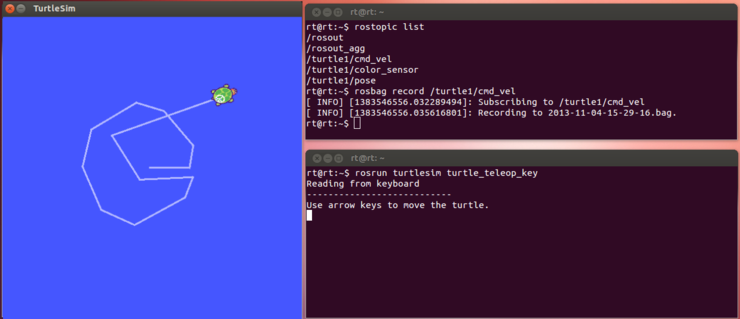
\includegraphics[width=0.8\columnwidth]{pictures/chapter5/rosbag_record.png}
\caption{rosbag record 예제}
\end{figure}

\begin{lstlisting}[language=ROS]
$ rosbag record -a
[ INFO] [1383547478.578148917]: Recording to 2013-11-04-15-44-38.bag.
[ INFO] [1383547479.577915716]: Subscribing to /turtle1/color_sensor
[ INFO] [1383547479.578655855]: Subscribing to /rosout
[ INFO] [1383547479.579363447]: Subscribing to /rosout_agg
[ INFO] [1383547479.579924366]: Subscribing to /turtle1/cmd_vel
[ INFO] [1383547479.580483400]: Subscribing to /turtle1/pose
\end{lstlisting}

\noindent
특정 토픽이 아닌 모든 토픽을 기록하고 싶다면 위와 같이 옵션에 "-a" 를 붙여주면 모든 토픽이 동시에 기록된다.

\vspace{\baselineskip}
\noindent
\stepcounter{num}\circled{\thenum} rosbag info [bag파일이름] : 배그파일의 정보를 확인한다

\begin{lstlisting}[language=ROS]
$ rosbag info 2013-11-04-15-29-16.bag 
path:        2013-11-04-15-29-16.bag
version:     2.0
duration:    16.9s
start:       Nov 04 2013 15:29:19.83 (1383546559.83)
end:         Nov 04 2013 15:29:36.74 (1383546576.74)
size:        23.1 KB
messages:    173
compression: none [1/1 chunks]
types:       geometry_msgs/Twist [9f195f881246fdfa2798d1d3eebca84a]
topics:      /turtle1/cmd_vel   173 msgs    : geometry_msgs/Twist
\end{lstlisting}

\noindent
배그파일의 정보를 확인할 수 있다. 위의 예제에서는 "/turtle1/cmd\_vel" 토픽을 기록하였으며, 총 173개의 메시지가 기록되었다. 사용된 메시지 형태는 "geometry\_msgs/Twist" 이며, 그이외에도 경로, bag 버전, 시간 등의 정보를 확인 할 수 있다.

\vspace{\baselineskip}
\noindent
\stepcounter{num}\circled{\thenum} rosbag play [bag파일이름] : 지정한 배그파일을 재생한다

\begin{lstlisting}[language=ROS]
$ rosbag play 2013-11-04-15-29-16.bag 
[ INFO] [1383548100.180862433]: Opening 2013-11-04-15-29-16.bag

Waiting 0.2 seconds after advertising topics... done.

Hit space to toggle paused, or 's' to step.

[RUNNING]  Bag Time: 1383546576.681423   Duration: 16.855905 / 16.918187     
Done.
\end{lstlisting}

\noindent
기록해둔 "2013-11-04-15-29-16.bag" 를 재생하는 명령어이다. 아래의 그림처럼 원본과 재생시의 데이터가 같음을 확인할 수 있다.

\begin{figure}[h]
\centering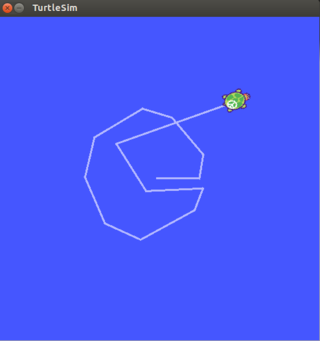
\includegraphics[width=0.4\columnwidth]{pictures/chapter5/rosbag_play1.png}
\centering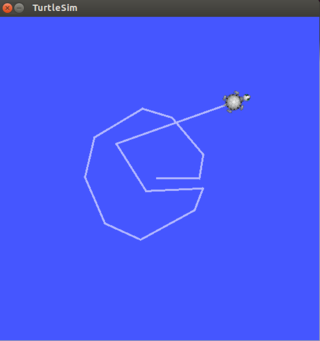
\includegraphics[width=0.4\columnwidth]{pictures/chapter5/rosbag_play2.png}
\caption{rosbag play 예제}
\end{figure}

\vspace{\baselineskip}
\noindent
\stepcounter{num}\circled{\thenum} rosbag compress [bag파일이름] : 지정한 배그파일을 압축한다

\begin{lstlisting}[language=ROS]
$ rosbag compress 2013-11-04-15-29-16.bag 
 2013-11-04-15-29-16.bag                     100%             16.4 KB 00:00  
\end{lstlisting}

\noindent
짧은 시간의 배그파일은 경우에는 그다지 용량이 크지 않아 문제 없지만, 장시간의 데이터를 기록할시에는 저장공간을 많이 차지한다. 위 압축 명령은 이럴때 사용하는 명령어로 압축해놓으면 매우 적은 저장 공간을 차지하게 된다. 위의 예제에서는 아래와 같이 1/3로 축소되었다. 그리고, 압축전 원본 파일은 orig라는 이름이 추가되어 별도로 저장된다.

\vspace{\baselineskip}
\noindent
/home/rt/2013-11-04-15-29-16.bag 8.6kB\\
/home/rt/2013-11-04-15-29-16.orig.bag 23.7kB

\vspace{\baselineskip}
\noindent
\stepcounter{num}\circled{\thenum} rosbag decompress [bag파일이름] : 지정한 배그파일을 압축해제한다

\begin{lstlisting}[language=ROS]
$ rosbag decompress 2013-11-04-15-29-16.bag 
2013-11-04-15-29-16.bag                     100%             16.3 KB 00:00  
\end{lstlisting}

\noindent
압축해제시에는 위의 명령어를 이용하면 된다. 압축전 상태로 원상 복귀된다.


% rosbag filter [입력bag파일] [출력bag파일] [옵션] : 지정된 내용을 제거한 새로운 bag 파일을 생성한다
% rosbag reindex [bag파일이름] : 인덱스를 재색인한다
% rosbag check [bag파일이름] : 지정한 배그파일이 현재 시스템에서 재생 가능한지 확인한다
% rosbag fix [입력bag파일] [출력bag파일] [옵션] : 버전이 다른 재생 불가능 bag파일을 재생가능하게 수정한다

%-------------------------------------------------------------------------------